

\newpage
\section{18-03-2019: ECCEZIONI}
\textbf{ECCEZIONI} \newline
Quando si lanciano eccezioni è bene ricordasi la differenza tra \textit{throw} e \textit{throws}
\begin{lstlisting}
public void writeList() throws IOException {
	if(true)
		 throw new IOException("demo"); 
}
\end{lstlisting}
\textbullet\ throws viene messa affianco alla firma del metodo, seguita da una lista delle eccezioni, e serve per dichiarare quali \textit{TIPI} di eccezioni possono essere lanciate da un determinato metodo. \newline
\textbullet\ throw seguito da un oggetto di tipo eccezione, serve per lanciare l'eccezione. \newline
Si noti quindi che con throws si dichiarano i tipi che verranno lanciati ma poi lanciamo oggetti: questo rappresenta un tipo di subtyping.
\newline
Si possono lanciare solo eccezione figlie del tipo \textit{Throwable}. Throwable è un super tipo di Exception e di tutte le classi lanciabili. \newline
Come regola generale quindi throw ha bisogno di essere seguito da un'espressione con tipo compatibile per poter essere lanciata.\newline
Il catch è lo strumento di binding per il throw. \newline
Le eccezioni non ritornano  per forza al chiamante se ritornano a chi se le prende. Infatti quando avviene una chiamata ad un metodo, questa appartiene ad una catena di chiamanti. Le eccezzioni possono quindi restituire qualcosa o al chiamante della funzione o ritornare qualcosa ad uno dei chiamanti della catena. Se risalendo questa catena l'eccezione non viene catturata nemmeno dal main questa passa direttamente alla \textit{Java Virtual Machine}\newline
Il sistema try-catch è stato ideato per evitare delle forti anomalie del programma. \newline
Nel canale ufficiale del return vengo solamente ritornati i risultati "giusti", in caso contrario verrà lanciata un'eccezione: questo è lo stile richiesto per i linguaggi evoluti. Invece di complicare il tipo di ritorno usiamo le eccezioni. \newline
Al posto delle eccezioni possiamo definire  un tipo di ritorno che codifica il fatto che hai trovato o meno quello che cercavi. Questa tecnica non è molto leggibile per chi non ha scritto il codice, sarebbe meglio usare il design pattern " tipo-eccezione". Esso è utile anche perchè in questo modo non si può scrivere codice che non funzioni, mentre definendo un nuovo tipo è possibile.


\noindent \textbf{I TRE TIPI DI ECCEZIONE} \newline
\textbullet\ Checked exception: Sono le condizioni di errore che l'utente deve poi obbligatoriamente gestire. Esse si usano per situazioni eccezionali in cui l'utente può ragionevolmente gestire il tutto con i try catch (ad esempio una selezione invalida in una interfaccia grafica).Questi tipi di errori devono necessariamente usare la clausola throws. \newline
\textbullet\ Runtime exception: Sono le condizioni di errore a gestione non obbligatoria, che se non gestite, possono arrivare fino al main e chiudere il programma. Sono usate per quegli errori non recuperabili con la gestione try e catch e che si possono evitare prestando attenzione quando si scrive il codice (es: index out of bound exception). Questi tipi di errori NON devono necessariamente usare la clausola throws.\newline
\textbullet\ Errors: Sono quegli errori irrecuperabili che l'utente non può gestire (memoria finita) \newline

\begin{center}
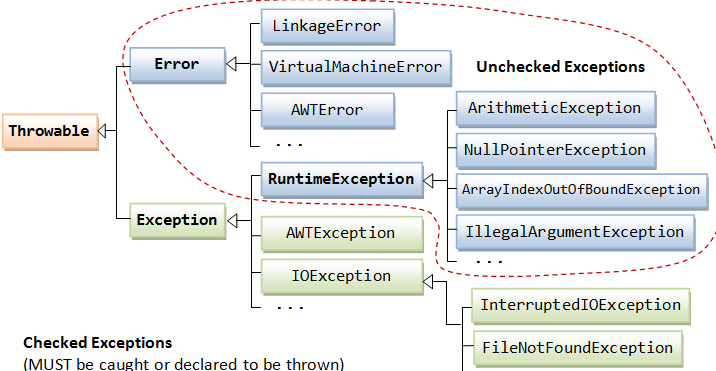
\includegraphics[width=%
0.6\textwidth]{eccezioni}
\end{center} 
\newpage






